\begin{comment}
\addbibresource{referencias/Referencias.bib}
\end{comment}

\section{Anexos}
\label{sc:anexos}

\begin{figure}
	\centering
	\sffamily
	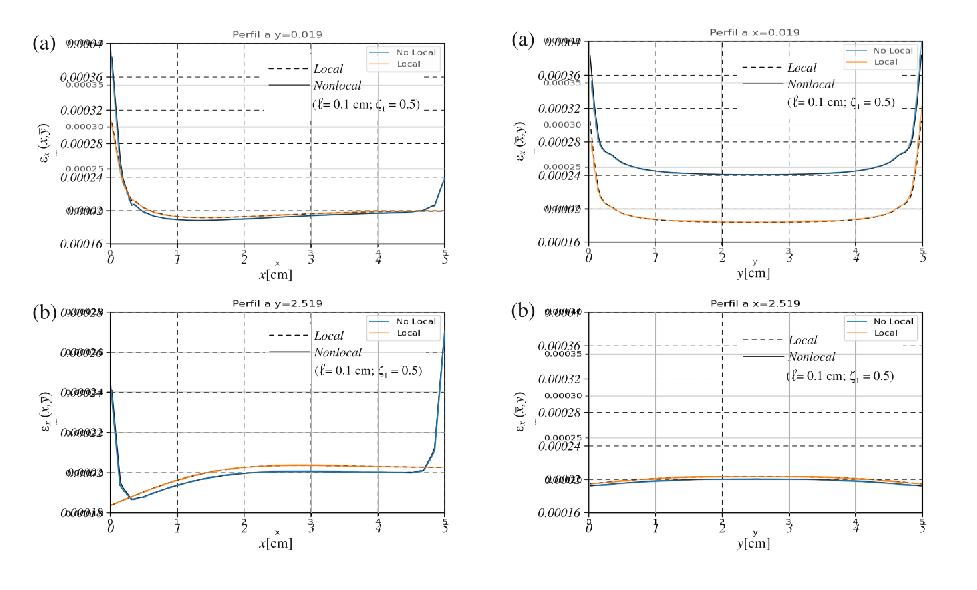
\includegraphics[width=\textwidth]{figuras/anexo_validacion.pdf}
	\caption{Gráficas de validación}
	\label{fig:anexos.validacion}
\end{figure}
\begin{eqfloat}

\begin{subequations}
	\begin{equation}
		\boldsymbol{UV_{nm}^{nloc}}[i,j]=t^2\int_{\Omega_n}\int_{\Omega_m}{A(\rho)\left[C_{12}\frac{\partial \psi_i^{l}}{\partial x}\frac{\partial \psi_j^{nl}}{\partial y}+C_{66}\frac{\partial \psi_i^{l}}{\partial y}\frac{\partial \psi_j^{nl}}{\partial x}\right]}{d\Omega_m}{d\Omega_n}
	\end{equation}
	\begin{equation}
		\boldsymbol{VU_{nm}^{nloc}}[i,j]=t^2\int_{\Omega_n}\int_{\Omega_m}{A(\rho)\left[C_{12}\frac{\partial \psi_i^{l}}{\partial y}\frac{\partial \psi_j^{nl}}{\partial x}+C_{66}\frac{\partial \psi_i^{l}}{\partial x}\frac{\partial \psi_j^{nl}}{\partial y}\right]}{d\Omega_m}{d\Omega_n}
	\end{equation}
	\begin{equation}
		\boldsymbol{VV_{nm}^{nloc}}[i,j]=t^2\int_{\Omega_n}\int_{\Omega_m}{A(\rho)\left[C_{11}\frac{\partial \psi_i^{l}}{\partial y}\frac{\partial \psi_j^{nl}}{\partial y}+C_{66}\frac{\partial \psi_i^{l}}{\partial x}\frac{\partial \psi_j^{nl}}{\partial x}\right]}{d\Omega_m}{d\Omega_n}
	\end{equation}
\end{subequations}
	\caption{Modelo de elementos finitos segun la terminología de \cite{Reddy}}
	\label{eq:anexos.matrices_elementos}
\end{eqfloat}